\documentclass[letterpaper,10pt]{article}

\usepackage{amstext}
\usepackage[fleqn]{amsmath}
\usepackage{MnSymbol}
\usepackage{listings}
\usepackage[letterpaper,margin=0.75in]{geometry}
\usepackage{float}
\usepackage{graphicx}
\usepackage{lastpage}
\usepackage{setspace}
\usepackage[amssymb]{SIunits}
\usepackage[titletoc]{appendix}
\usepackage{pdfpages}
\usepackage{fancyhdr}
\usepackage{subfig}
\usepackage{color}
\usepackage{cancel}
\usepackage{pdfpages}
\usepackage{hyperref}

\hypersetup{
    bookmarks=true,         % show bookmarks bar?
    unicode=false,          % non-Latin characters in Acrobat’s bookmarks
    pdftoolbar=true,        % show Acrobat’s toolbar?
    pdfmenubar=true,        % show Acrobat’s menu?
    pdffitwindow=true,     % window fit to page when opened
    pdfstartview={FitH},    % fits the width of the page to the window
    pdftitle={Heat Conduction Through Rectangular Domain},    % title
    pdfauthor={Kenton Hamaluik},     % author
    pdfsubject={Finite Element Analysis Using Deal.II},   % subject of the document
    pdfcreator={Kenton Hamaluik},   % creator of the document
    pdfnewwindow=true,      % links in new window
    colorlinks=true,       % false: boxed links; true: colored links
    linkcolor=black,          % color of internal links
    citecolor=black,        % color of links to bibliography
    filecolor=black,      % color of file links
    urlcolor=black           % color of external links
}

\definecolor{dkgreen}{rgb}{0,0.6,0}
\definecolor{gray}{rgb}{0.5,0.5,0.5}
\definecolor{mauve}{rgb}{0.58,0,0.82}
 
\lstset{ %
	language=C++,                   % the language of the code
	basicstyle=\footnotesize,       % the size of the fonts that are used for the code
	numbers=left,                   % where to put the line-numbers
	numberstyle=\tiny\color{gray},  % the style that is used for the line-numbers
	stepnumber=1,                   % the step between two line-numbers. If it's 1, each line 
								    % will be numbered
	numbersep=5pt,                  % how far the line-numbers are from the code
	backgroundcolor=\color{white},  % choose the background color. You must add \usepackage{color}
	showspaces=false,               % show spaces adding particular underscores
	showstringspaces=false,         % underline spaces within strings
	showtabs=false,                 % show tabs within strings adding particular underscores
	frame=single,                   % adds a frame around the code
	rulecolor=\color{black},        % if not set, the frame-color may be changed on line-breaks within not-black text (e.g. commens (green here))
	prebreak=\raisebox{0ex}[0ex][0ex]{\ensuremath{\rhookswarrow}},
	postbreak=\raisebox{0ex}[0ex][0ex]{\ensuremath{\rcurvearrowse\space}},
	tabsize=4,                      % sets default tabsize to 2 spaces
	captionpos=t,                   % sets the caption-position to bottom
	breaklines=true,                % sets automatic line breaking
	breakatwhitespace=true,         % sets if automatic breaks should only happen at whitespace
	title=\lstname,                 % show the filename of files included with \lstinputlisting;
								    % also try caption instead of title
	keywordstyle=\color{blue},      % keyword style
	commentstyle=\color{dkgreen},   % comment style
	stringstyle=\color{mauve},      % string literal style
	escapeinside={\%*}{*)},         % if you want to add a comment within your code
	morekeywords={*,...},           % if you want to add more keywords to the set
}

\renewcommand{\arraystretch}{1.5}

\newcommand{\HRule}{\rule{\linewidth}{0.5mm}}

\pagestyle{empty}

\begin{document}
\begin{center}
\vspace*{\fill}
\HRule \\[0.5cm]
\textsc{\LARGE MecE 663}\\
\textsc{\Large Project:}\\
\textsc{\large Heat Conduction Through Rectangular Domain}\\
\HRule \\[0.7cm]
Kenton Hamaluik\\[0.5cm]
April 18, 2012\\
Instructor: Dr. Marc Secanell Gallart\\
University of Alberta
\vspace*{\fill}
\end{center}
\pagebreak

\tableofcontents
\pagebreak
\listoffigures
\listoftables
\pagebreak

\pagestyle{fancyplain}
\fancyhf{}
\lhead{April 18, 2012 \\}
\chead{MecE 663 \\ Term Project}
\rhead{Hamaluik, Kenton \\ 1142840}
\rfoot{Page \thepage}
\setcounter{page}{1}

\section{Problem Definition}
\label{sec:definition}
The goal of this problem is determine the temperature distribution throughout a rectangular domain as given in figure \ref{fig:domain}. The temperature distribution is defined by the partial differential equation (PDE) given in equation \ref{equ:pde}.

\begin{figure}[H]
	\centering
	\includegraphics[width=0.6\textwidth]{domain.png}
	\caption{Problem domain and boundaries}
	\label{fig:domain}
\end{figure}

\begin{equation}
\label{equ:pde}
\frac{\partial}{\partial x}\left(k_x\frac{\partial T}{\partial x}\right) + \frac{\partial}{\partial y}\left(k_y\frac{\partial T}{\partial y}\right) + f(x,y) = 0
\end{equation}

\noindent where the problem domain is $\Omega \in \unit{\left(\left(0,0\right),\left(1,2.5\right)\right)}{m}$, $f(x,y)$ is as defined in equation \ref{equ:f}, and the constant thermal conductivity coefficients are given as:
\begin{equation}
\label{equ:f}
f(x,y) = Ax^2 \unit{}{W/m^3}
\end{equation}
\[k_x(x,y)=\unit{15}{W/m\usk K}\]
\[k_y(x,y)=\unit{25}{W/m\usk K}\]

\noindent In equation \ref{equ:f}, $A$ represents a variable heat generation term whose effect is to be investigated with:
\[A \in \unit{(0, 5)}{kW/m^5}\]

\noindent In this problem, there are three distinct sets of boundary conditions (illustrated in figure \ref{fig:domain}):
\begin{enumerate}
	\item A variable heat flux along $\partial \Omega_1$ subject to the following conditions:
	\[k_x\frac{\partial T}{\partial x} = B \left(1-y\right) \unit{}{W/m^2}\]
	\[k_y\frac{\partial T}{\partial y} = 0 \unit{}{W/m^2}\]
	Where:
	\[B = \unit{50}{W/m^3}\]
	
	\item An adiabatic boundary condition (heat flux of 0) along $\partial \Omega_2$ such that the following holds on this boundary:
	\[k_x\frac{\partial T}{\partial x} = 0 \unit{}{W/m^2}\]
	\[k_y\frac{\partial T}{\partial y} = 0 \unit{}{W/m^2}\]
	
	\item A constant Dirichlet boundary condition along $\partial \Omega_3$ where:
	\[T = \unit{400}{K}\]
\end{enumerate}

\section{Development of the Weak Form of the Problem}
To develop the weak weak form of the problem, the PDE given in equation \ref{equ:pde} is multiplied by a weighting function $w(x,y)$ and integrated over the domain such that:
\[\int_\Omega w \left[\frac{\partial}{\partial x}\left(k_x\frac{\partial T}{\partial x}\right) + \frac{\partial}{\partial y}\left(k_y\frac{\partial T}{\partial y}\right) + f(x,y)\right] d\Omega = 0\]
\noindent or:
\begin{equation}
\label{equ:wintpde}
-\int_\Omega w \left[\frac{\partial}{\partial x}\left(k_x\frac{\partial T}{\partial x}\right) + \frac{\partial}{\partial y}\left(k_y\frac{\partial T}{\partial y}\right)\right] d\Omega = \int_\Omega wf(x,y)d\Omega
\end{equation}

\noindent Now we must apply integration by parts (in 2-dimensions) to ``weaken'' the second-derivative terms in equation \ref{equ:wintpde} such that both the solution and weighting functions belong to $\mathrm{H}^1$, noting that in general:
\[\int_\Omega w \frac{\partial G}{\partial x}d\Omega = -\int_\Omega \frac{\partial w}{\partial x}Gd\Omega + \oint_\Gamma n_xwGd\Gamma\]
\noindent where in our equation (in the $x$ direction),
\[G = k_x\frac{\partial T}{\partial x}\]
\noindent and:
\[\begin{array}{l}
\Gamma = d\Omega \\
n_x = \left(1,0\right) \cdot \vec{n} \\
n_y = \left(0,1\right) \cdot \vec{n} \\
\vec{n} = \text{surface norm of } \Gamma
\end{array}\]
\noindent Such that:
\[\begin{split}
	\int_\Omega w \frac{\partial G}{\partial x}d\Omega &= -\int_\Omega \frac{\partial w}{\partial x}Gd\Omega + \oint_\Gamma n_xwGd\Gamma \\
	\int_\Omega w \frac{\partial}{\partial x}\left(k_x\frac{\partial T}{\partial x}\right)d\Omega &= -\int_\Omega \frac{\partial w}{\partial x}\left(k_x\frac{\partial T}{\partial x}\right)d\Omega + \oint_\Gamma n_xw\left(k_x\frac{\partial T}{\partial x}\right)d\Gamma
\end{split}\]
\noindent We note that this formulation is identical in the $y$ direction, so:
\[\int_\Omega w \frac{\partial}{\partial y}\left(k_y\frac{\partial T}{\partial y}\right)d\Omega = -\int_\Omega \frac{\partial w}{\partial y}\left(k_x\frac{\partial T}{\partial y}\right)d\Omega + \oint_\Gamma n_yw\left(k_y\frac{\partial T}{\partial y}\right)d\Gamma\]

\noindent We can now combine these results with the problem given in equation \ref{equ:wintpde} to weaken the second-derivative terms:
\[-\left\{-\int_\Omega \left[\frac{\partial w}{\partial x}\left(k_x\frac{\partial T}{\partial x}\right) + \frac{\partial w}{\partial y}\left(k_y\frac{\partial T}{\partial y}\right) \right]d\Omega + \oint_\Gamma \left[n_xw\left(k_x\frac{\partial T}{\partial x}\right) + n_yw\left(k_y\frac{\partial T}{\partial y}\right)\right]d\Gamma\right\} = \int_\Omega wf(x,y)d\Omega\]
\[\int_\Omega \left[\frac{\partial w}{\partial x}\left(k_x\frac{\partial T}{\partial x}\right) + \frac{\partial w}{\partial y}\left(k_y\frac{\partial T}{\partial y}\right) \right]d\Omega - \oint_\Gamma \left[n_xw\left(k_x\frac{\partial T}{\partial x}\right) + n_yw\left(k_y\frac{\partial T}{\partial y}\right)\right]d\Gamma = \int_\Omega wf(x,y)d\Omega\]
\noindent Leaving us with the weak formulation of the problem:
\begin{equation}
\label{equ:weak}
\boxed{\int_\Omega \left[\frac{\partial w}{\partial x}\left(k_x\frac{\partial T}{\partial x}\right) + \frac{\partial w}{\partial y}\left(k_y\frac{\partial T}{\partial y}\right) \right]d\Omega = \int_\Omega wf(x,y)d\Omega + \oint_\Gamma \left[n_xw\left(k_x\frac{\partial T}{\partial x}\right) + n_yw\left(k_y\frac{\partial T}{\partial y}\right)\right]d\Gamma}
\end{equation}

\subsection{Formation of the Element-Wise System Matrix and Right Hand Side}
Using the Bubnov-Galerkin approximation functions (where $m$ is the number of degrees of freedom in the problem),
\begin{equation}
\label{equ:bubnov-galerkin}
\begin{array}{l}
T(x,y) = \displaystyle\sum\limits_{j=1}^m \tau_j \phi_j(x,y) \\
w(x,y) = \displaystyle\sum\limits_{i=1}^m \omega_i \phi_i(x,y) \\
\end{array}
\end{equation}
\noindent we can rearrange the weak form of the problem given in equation \ref{equ:weak} to solve for the unknown temperature distribution coefficients, $\tau_j$ (also noting that for the element-wise system equations we can disregard the boundary terms):
\[\begin{split}
\int_\Omega \left[\frac{\partial w}{\partial x}\left(k_x\frac{\partial T}{\partial x}\right) + \frac{\partial w}{\partial y}\left(k_y\frac{\partial T}{\partial y}\right) \right]d\Omega &= \int_\Omega wf(x,y)d\Omega + \cancelto{0}{\oint_\Gamma \left[n_xw\left(k_x\frac{\partial T}{\partial x}\right) + n_yw\left(k_y\frac{\partial T}{\partial y}\right)\right]d\Gamma} \\
\int_\Omega \left[\displaystyle\sum\limits_{i=1}^m \omega_i\frac{\partial \phi_i}{\partial x}\left(k_x\displaystyle\sum\limits_{j=1}^m\tau_j\frac{\partial \phi_j}{\partial x}\right) + \displaystyle\sum\limits_{i=1}^m \omega_i\frac{\partial \phi_i}{\partial y}\left(k_y\displaystyle\sum\limits_{j=1}^m\tau_j\frac{\partial \phi_j}{\partial y}\right) \right]d\Omega &= \int_\Omega \displaystyle\sum\limits_{i=1}^m \omega_i\phi_if(x,y)d\Omega
\end{split}\]

\noindent This constitutes a system of equations which can be represented using matrix notation: $\mathbf{K}\mathbf{\tau}=\mathbf{F}$ where each equation is defined as:
\[
\int_\Omega \left[ \omega_i\frac{\partial \phi_i}{\partial x}\left(k_x\tau_j\frac{\partial \phi_j}{\partial x}\right) +  \omega_i\frac{\partial \phi_i}{\partial y}\left(k_y\tau_j\frac{\partial \phi_j}{\partial y}\right) \right]d\Omega = \int_\Omega \omega_i\phi_if(x,y)d\Omega
\]
Since the $\omega_i$s and $\tau_j$s are all constant, we can cancel the $\omega_i$s which appear on both sides of the equation and rearrange to solve for $\tau_j$:
\[\begin{split}
\int_\Omega \left[ \cancel{\omega_i}\frac{\partial \phi_i}{\partial x}\left(k_x\tau_j\frac{\partial \phi_j}{\partial x}\right) +  \cancel{\omega_i}\frac{\partial \phi_i}{\partial y}\left(k_y\tau_j\frac{\partial \phi_j}{\partial y}\right) \right]d\Omega &= \int_\Omega \cancel{\omega_i}\phi_if(x,y)d\Omega
\\
\left\{\int_\Omega \left[ \frac{\partial \phi_i}{\partial x}\left(k_x\frac{\partial \phi_j}{\partial x}\right) + \frac{\partial \phi_i}{\partial y}\left(k_y\frac{\partial \phi_j}{\partial y}\right) \right]d\Omega\right\}\tau_j &= \int_\Omega \phi_if(x,y)d\Omega
\end{split}\]
\noindent such that the elements of the $\mathbf{K}$ system matrix are defined as:
\begin{equation}
\label{equ:Kij}
\boxed{\mathbf{K}_{ij} = \int_\Omega \left[ \frac{\partial \phi_i}{\partial x}\left(k_x\frac{\partial \phi_j}{\partial x}\right) + \frac{\partial \phi_i}{\partial y}\left(k_y\frac{\partial \phi_j}{\partial y}\right) \right]d\Omega}
\end{equation}
\noindent and the elements of $\mathbf{F}$ right hand side are defined as:
\begin{equation}
\label{equ:Fi}
\boxed{\mathbf{F}_i = \int_\Omega \phi_if(x,y)d\Omega}
\end{equation}
(or)
\[\mathbf{F}_i = \int_\Omega \phi_iAx^2d\Omega\]

\subsection{Application of the Weak Form Neumann Boundary Conditions}
Now we consider the Bubnov-Galerkin approximation of the Neumann boundary conditions that will be applied to the right hand side, through the boundary term expression:
\[
\mathbf{F}_\Gamma = \oint_\Gamma \left[n_xw\left(k_x\frac{\partial T}{\partial x}\right) + n_yw\left(k_y\frac{\partial T}{\partial y}\right)\right]d\Gamma
\]
\noindent Applying the Bubnov-Galerkin approximation functions given in equation \ref{equ:bubnov-galerkin} to the above boundary terms yields:
\[
\mathbf{F}_\Gamma = \oint_\Gamma \left[n_x\displaystyle\sum\limits_{i=1}^m\omega_i\phi_i\left(k_x\frac{\partial T}{\partial x}\right) + n_y\displaystyle\sum\limits_{i=1}^m\omega_i\phi_i\left(k_y\frac{\partial T}{\partial y}\right)\right]d\Gamma
\]
\noindent where this is a system of equations and $\omega_i$ will cancel out as before:
\[
\mathbf{F}_{\Gamma,i} = \oint_\Gamma \left[n_x\phi_i\left(k_x\frac{\partial T}{\partial x}\right) + n_y\phi_i\left(k_y\frac{\partial T}{\partial y}\right)\right]d\Gamma
\]

\noindent This integral may then be further simplified by considering each boundary region in turn, with the right hand side $\mathbf{F}_i$ (given in equation \ref{equ:Fi}) being modified by $\mathbf{F}_{\Gamma,i}$ as:
\[
\boxed{\mathbf{F}_i = \mathbf{F}_i + \displaystyle\sum\limits_{b=1}^3 \mathbf{F}_{\Gamma_b,i}}
\]

\subsubsection{Boundary 1 (Heat Flux)}
Boundary 1 exists solely on the domain where $x=0$, with $y \in (0, 1)$, thus $\Gamma = y \in (0, 1)$ and $d\Gamma = dy$. Further, along this boundary, $\vec{n} = \left(-1,0\right)$ such that $n_x=-1$ and $n_y$ = 0. The right hand side contribution of the boundary term along this boundary thus becomes:
\[\mathbf{F}_{\Gamma_1,i} = -\int_0^1 \phi_i\left(k_x\frac{\partial T}{\partial x}\right)dy\]
We can now note the given boundary condition:
\[k_x\frac{\partial T}{\partial x} = B \left(1-y\right) \unit{}{W/m^2}\]
Such that the extra right hand side contribution along this boundary is:
\begin{equation}
\label{equ:F1i}
\boxed{\mathbf{F}_{\Gamma_1,i} = -\int_0^1 B \phi_i \left(1-y\right)dy}
\end{equation}

\subsubsection{Boundary 2 (Insulation)}
Along boundary 2, there is a prescribed insulated boundary, meaning that:
\[k_x\frac{\partial T}{\partial x} = \unit{0}{W/m^2}\]
\[k_y\frac{\partial T}{\partial y} = \unit{0}{W/m^2}\]
\noindent Thus straight away we can see that there will be zero contribution from the boundary terms along boundary 2:
\[
\mathbf{F}_{\Gamma_2,i} = \oint_\Gamma \left[n_x\phi_i\cancelto{0}{\left(k_x\frac{\partial T}{\partial x}\right)} + n_y\phi_i\cancelto{0}{\left(k_y\frac{\partial T}{\partial y}\right)}\right]d\Gamma
\]
\begin{equation}
\label{equ:F2i}
\boxed{\mathbf{F}_{\Gamma_2,i} = 0}
\end{equation}

\subsubsection{Boundary 3 (Constant Temperature)}
Along boundary 3 there is a constant Dirichlet boundary condition, meaning that the temperature along this boundary is already given. When a Dirichlet boundary condition is present, the solution does not have to be approximated and so the weighting function at the boundary is 0:
\[\phi_i = 0\]
\noindent Similar to the result in boundary 2 then, we can see that there will be zero contribution from the boundary terms along boundary 3:
\[
\mathbf{F}_{\Gamma_3,i} = \oint_\Gamma \left[n_x\cancelto{0}{\phi_i}\left(k_x\frac{\partial T}{\partial x}\right) + n_y\cancelto{0}{\phi_i}\left(k_y\frac{\partial T}{\partial y}\right)\right]d\Gamma
\]
\begin{equation}
\label{equ:F3i}
\boxed{\mathbf{F}_{\Gamma_3,i} = 0}
\end{equation}

\subsection{Numerical Integration Formulation}
In order to evaluate the integrals given in equations \ref{equ:Kij}, \ref{equ:Fi} and \ref{equ:F1i}, it is prudent to use numerical integration schemes that can be easily implemented in a computer. A common numerical integration scheme is to use Gauss-Legendre quadrature, where:
\begin{equation}
\label{equ:gauss_quadrature}
\int_{-1}^1 F(x)dx \approx \sum_{i=1}^mF(x_i)\cdot w_i
\end{equation}
\noindent where $x_i$ are weighting anchors that depend on $n$ and $w_i$ are weighting coefficients that also depend on $n$.

Unfortunately, to use this integration scheme, the integration limits must be $(-1,1)$. To achieve this, an iso-parametric mapping of the element domains must be done from their natural domains to the domain $\left((-1,-1),(1,1)\right)$. This mapping is performed through the functions:
\[X(\zeta,\eta) = \sum x_i \psi_i(\zeta,\eta)\]
\[Y(\zeta,\eta) = \sum y_i \psi_i(\zeta,\eta)\]
\noindent where $\psi_i$ are termed the ``shape functions'' for a given type and order of the elements used in the approximation.

Using this mapping, integrals over the element domain may be transferred into integrations over our numerical integration domain using:
\[
\int_{\Omega^e} f(x,y)d\Omega^e = \int_{\hat{\Omega}^e}f\left[X(\zeta,\eta),Y(\zeta,\eta)\right]\cdot\left|J(\zeta,\eta)\right|d\zeta d\eta
\]
\noindent where $\left|J(\zeta,\eta)\right|$ is the determinant of the Jacobian matrix and is defined as:
\[
\left|J(\zeta,\eta)\right| = \det \left[\begin{array}{cc}
\frac{\partial X}{\partial \zeta} & \frac{\partial Y}{\partial \zeta} \\
\frac{\partial X}{\partial \eta} & \frac{\partial Y}{\partial \eta} \\
\end{array}\right]
\]

Now, if we substitute this back into equation \ref{equ:gauss_quadrature}, we get that an integral over the 2-dimensional domain $\Omega$ can be approximated as such:
\begin{equation}
\label{equ:numint}
\begin{split}
	\int_{\Omega^e} f(x,y)d\Omega^e &= \int_{\hat{\Omega}^e}f\left[X(\zeta,\eta),Y(\zeta,\eta)\right]\cdot\left|J(\zeta,\eta)\right|d\zeta d\eta \\
	&= \int_{-1}^{1}\int_{-1}^1f\left[X(\zeta,\eta),Y(\zeta,\eta)\right]\cdot\left|J(\zeta,\eta)\right|d\zeta d\eta \\
	&\approx \sum_{i=1}^m\sum_{j=1}^n\left\{f\left[X(\zeta_i,\eta_j),Y(\zeta_i,\eta_j)\right]\cdot\left|J(\zeta_i,\eta_j)\right| \cdot w_j \right\}\cdot w_i
\end{split}
\end{equation}

Now, applying equation \ref{equ:numint} to equations \ref{equ:Kij}, \ref{equ:Fi} and \ref{equ:F1i}, we arrive at the following approximations:
\[\begin{split}
	\mathbf{K}_{ij} &= \int_\Omega \left[ \frac{\partial \phi_i}{\partial x}\left(k_x\frac{\partial \phi_j}{\partial x}\right) + \frac{\partial \phi_i}{\partial y}\left(k_y\frac{\partial \phi_j}{\partial y}\right) \right]d\Omega \\
	&= \int_{-1}^1\int_{-1}^1 \left[ \frac{\partial \phi_i\left(\zeta,\eta\right)}{\partial \zeta}\left(k_x\frac{\partial \phi_j\left(\zeta,\eta\right)}{\partial \zeta}\right) + \frac{\partial \phi_i\left(\zeta,\eta\right)}{\partial \eta}\left(k_y\frac{\partial \phi_j\left(\zeta,\eta\right)}{\partial \eta}\right) \right]\cdot\left|J\left(\zeta,\eta\right)\right|d\zeta d\eta
\end{split}\]
\begin{equation}
\label{equ:Kij_quad}
	\boxed{\mathbf{K}_{ij} \approx \sum_{p=1}^m\sum_{q=1}^n \left[\frac{\partial \phi_i\left(\zeta_p,\eta_q\right)}{\partial \zeta}\left(k_x\frac{\partial \phi_j\left(\zeta_p,\eta_q\right)}{\partial \zeta}\right) + \frac{\partial \phi_i\left(\zeta_p,\eta_q\right)}{\partial \eta}\left(k_y\frac{\partial \phi_j\left(\zeta_p,\eta_q\right)}{\partial \eta}\right) \right]\cdot\left|J\left(\zeta_i,\eta_j\right)\right|\cdot w_pw_q}
\end{equation}

\[\begin{split}
	\mathbf{F}_i &= \int_\Omega \phi_if(x,y)d\Omega \\
	&= \int_{-1}^1\int_{-1}^1 \phi_i\left(\zeta,\eta\right)f\left(X(\zeta,\eta),Y(\zeta,\eta)\right)\cdot \left|J\left(\zeta,\eta\right)\right|d\zeta d\eta \\
\end{split}\]
\begin{equation}
\label{equ:Fi_quad}
	\boxed{\mathbf{F}_i \approx \sum_{p=1}^m\sum_{q=1}^n\phi_i\left(\zeta_p,\eta_q\right)f\left(X(\zeta_p,\eta_q),Y(\zeta_p,\eta_q)\right)\cdot \left|J\left(\zeta_p,\eta_q\right)\right| \cdot w_jw_i}
\end{equation}

\[\begin{split}
	\mathbf{F}_{\Gamma_1,i} &= -\int_0^1 B \phi_i \left(1-y\right)dy \\
	&= \int_{-1}^1 B\phi_i\left(\eta\right)\left(1-Y(\eta)\right)\cdot \left|J\left(\zeta,\eta\right)\right|d\eta \\
\end{split}\]
\begin{equation}
\label{equ:F1i_quad}
	\boxed{\mathbf{F}_{\Gamma_1,i} \approx \sum_{q=1}^n B\phi_i\left(\eta_q\right)\left(1-Y(\eta_q)\right)\cdot \left|J\left(\zeta_p,\eta_q\right)\right|\cdot w_q}
\end{equation}

\section{Discretization of the Domain}
The domain can naturally be split into to two regions to accomodate the unique set of boundaries for this problem (see figure \ref{fig:domain} for boundary location information). A ``coarse'' grid which defines two elements and their appropriate boundaries is given in figure \ref{fig:grid_r0}.

\begin{figure}[H]
	\centering
	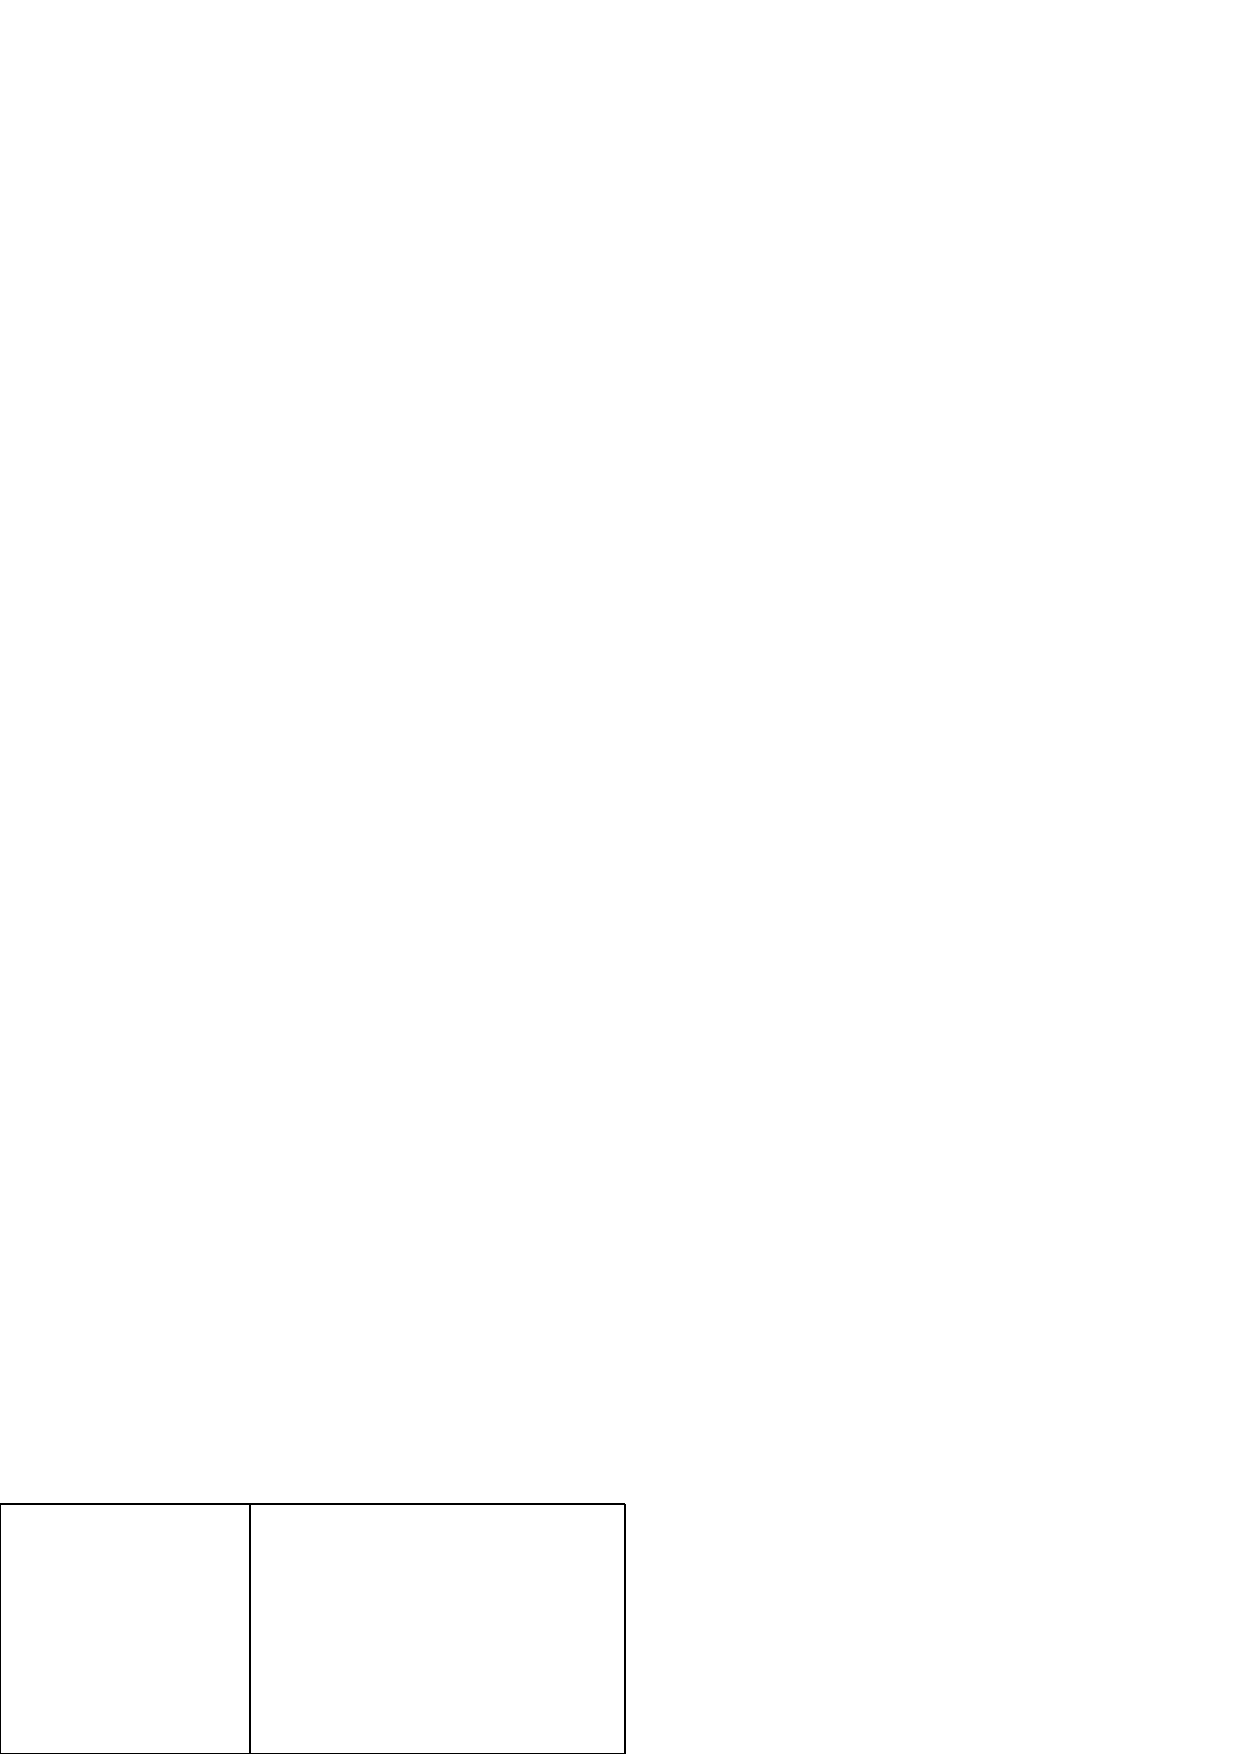
\includegraphics[width=0.5\textwidth]{mesh_r0.pdf}
	\caption{Coarse grid with only 2 elements}
	\label{fig:grid_r0}
\end{figure}

Such a coarse grid provides very little detail about the solution and is a poor approximation of the true temperature distribution throughout the problem domain. Subsequently, the mesh may be refined numerous times to provide greater granularity of the domain, allowing much more finely detailed solutions to be obtained. Structured mesh refinements resulting in 8, 32, 128, and 512 elements throughout the domain are given in figure \ref{fig:meshs}.

\begin{figure}[H]
	\centering
	\subfloat[1 mesh refinement, 8 elements]{\label{fig:mesh_1}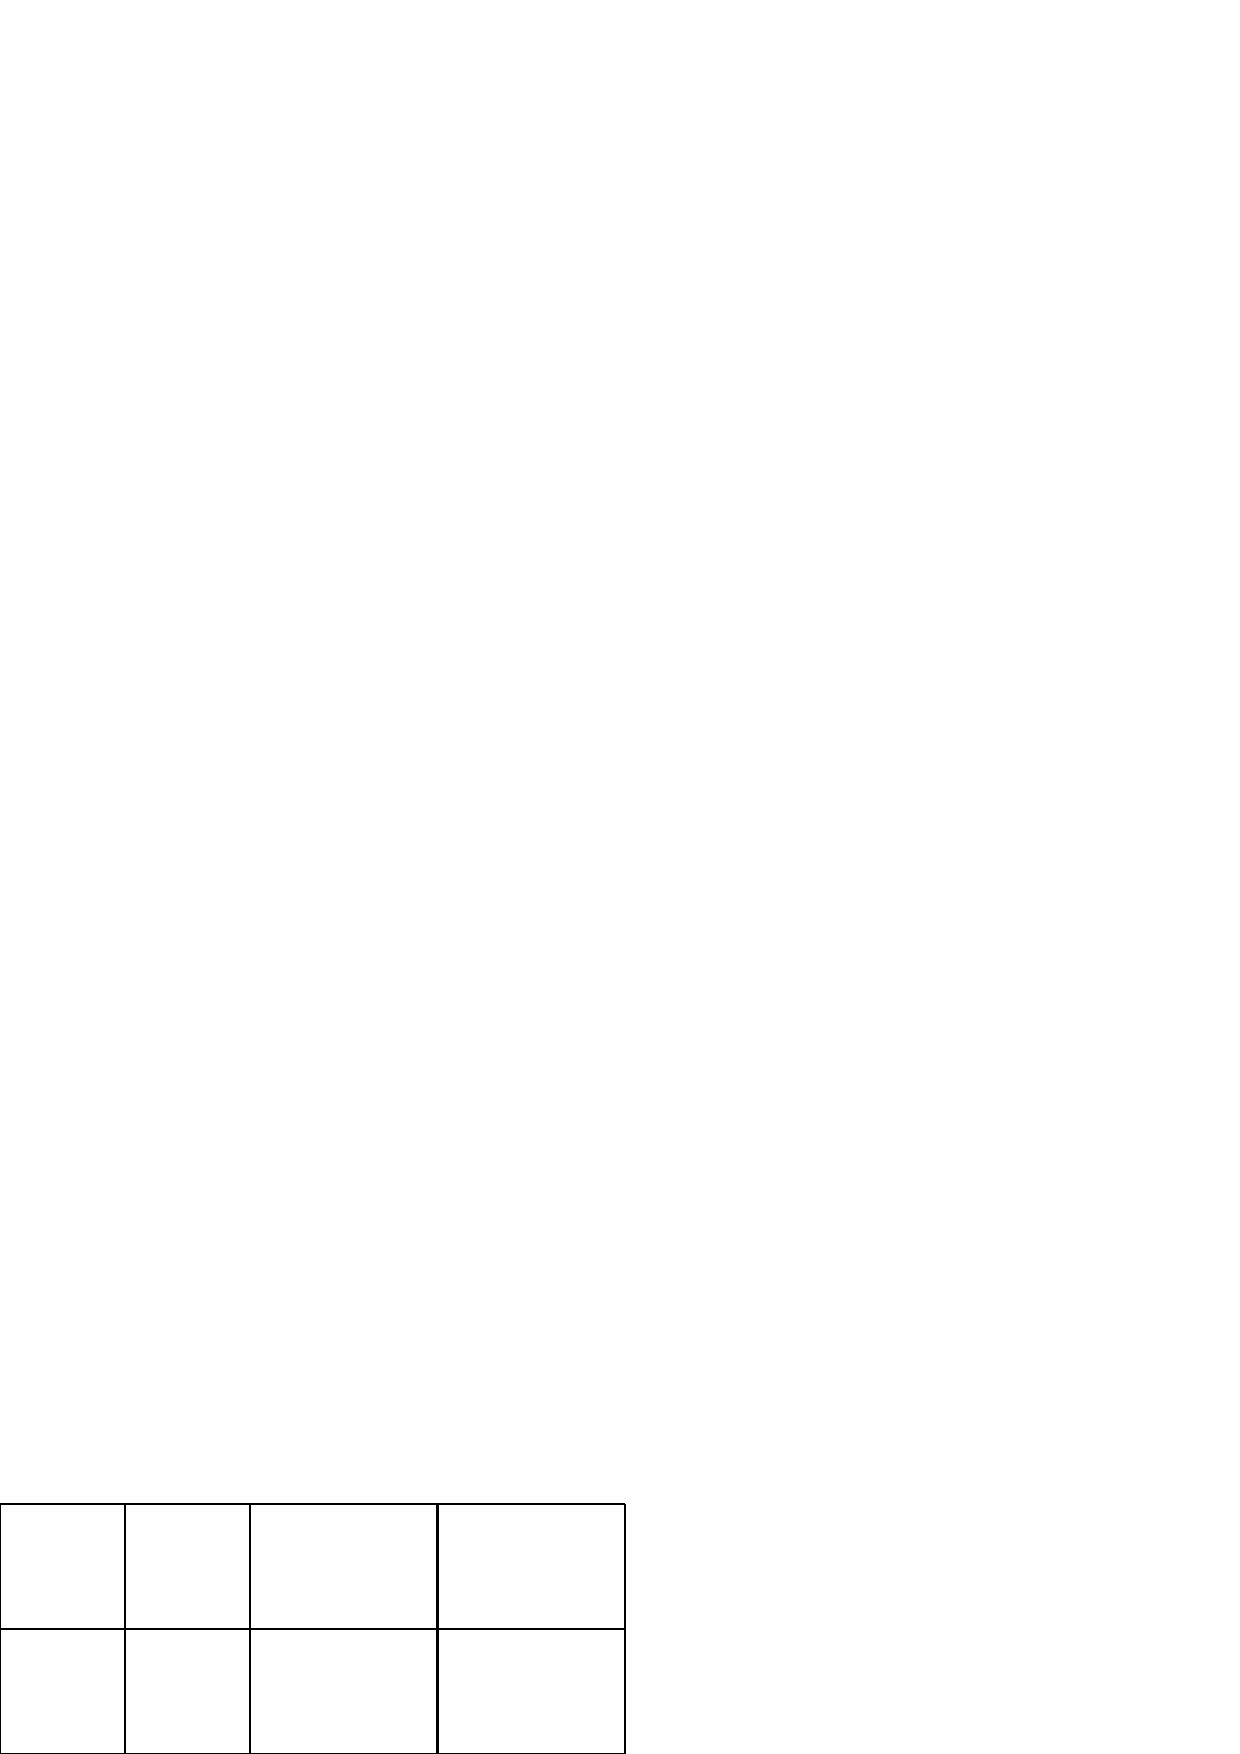
\includegraphics[width=0.45\textwidth]{mesh_r1.pdf}} \;
	\subfloat[2 mesh refinements, 32 elements]{\label{fig:mesh_2}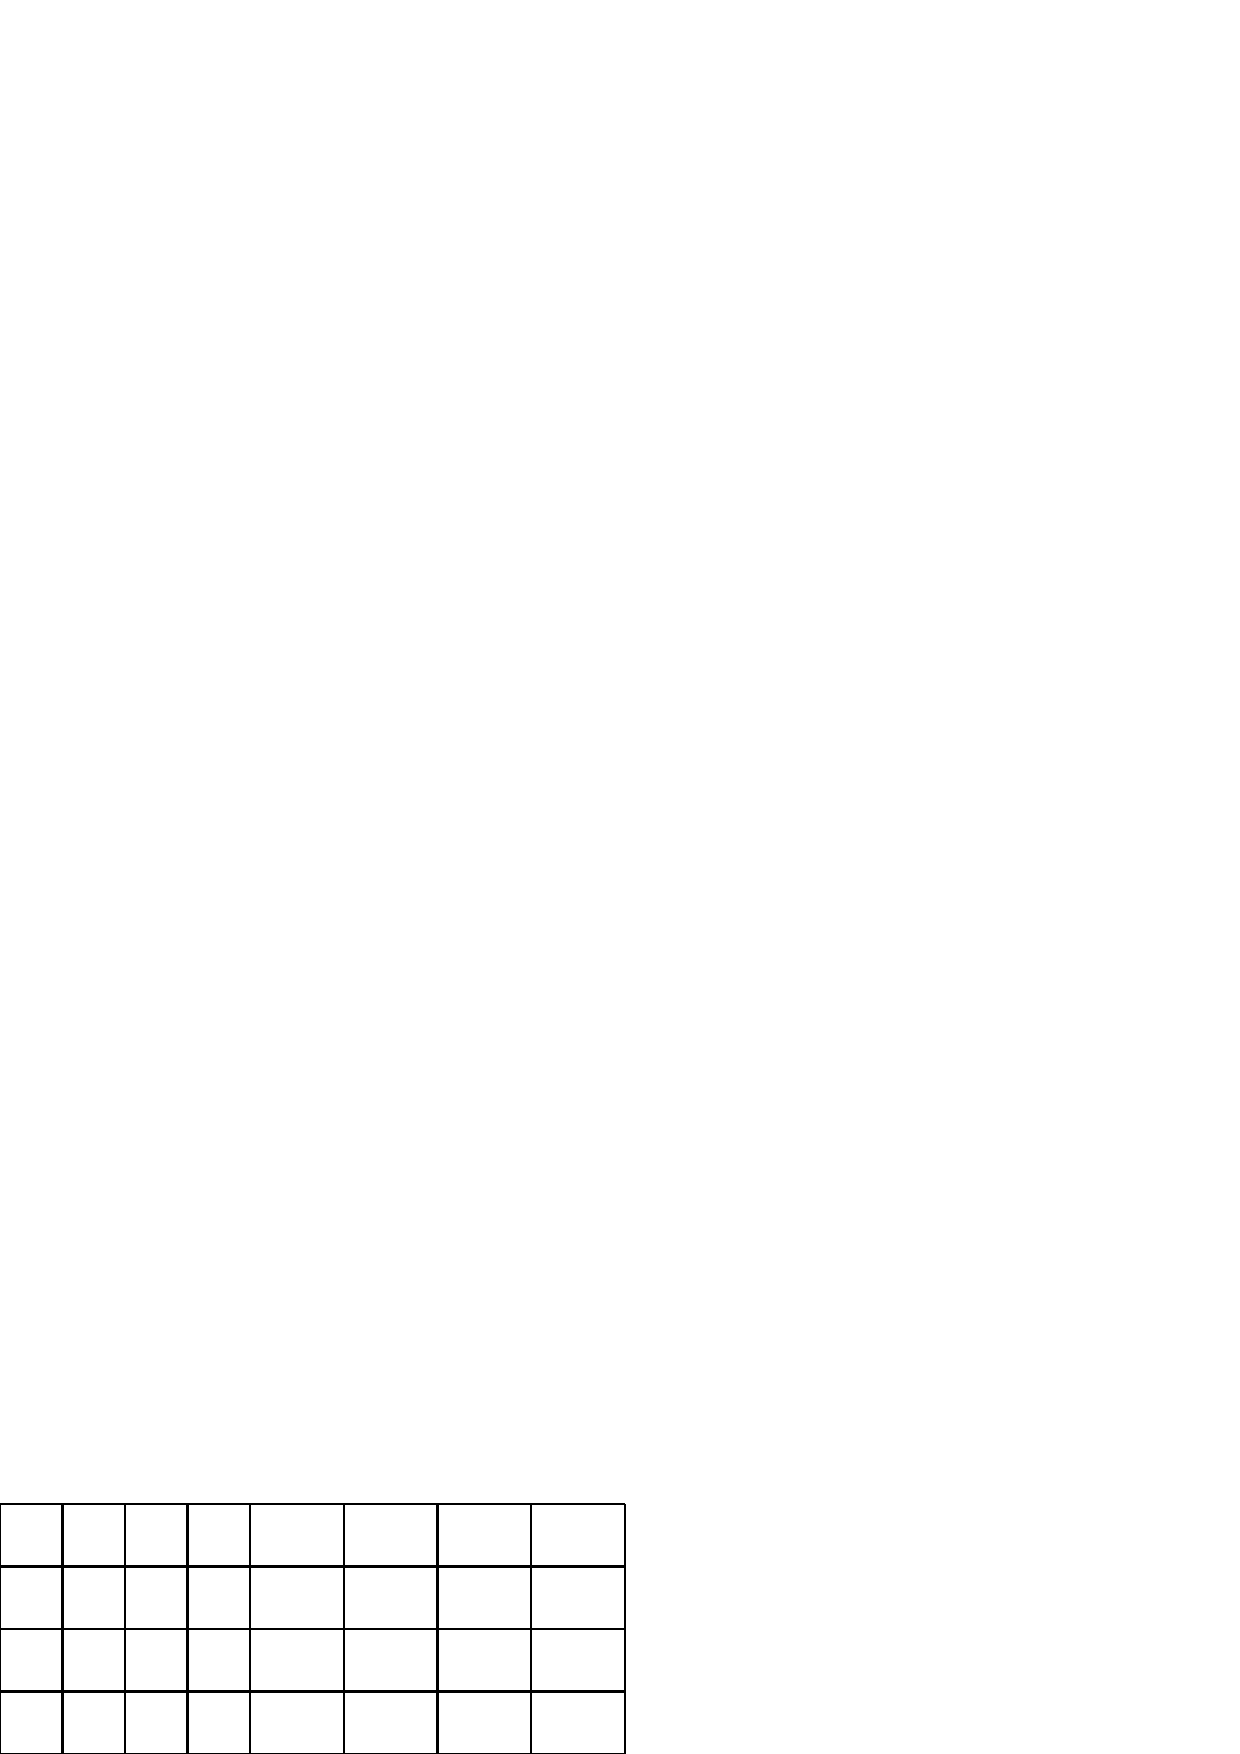
\includegraphics[width=0.45\textwidth]{mesh_r2.pdf}} \\
	\subfloat[3 mesh refinements, 128 elements]{\label{fig:mesh_3}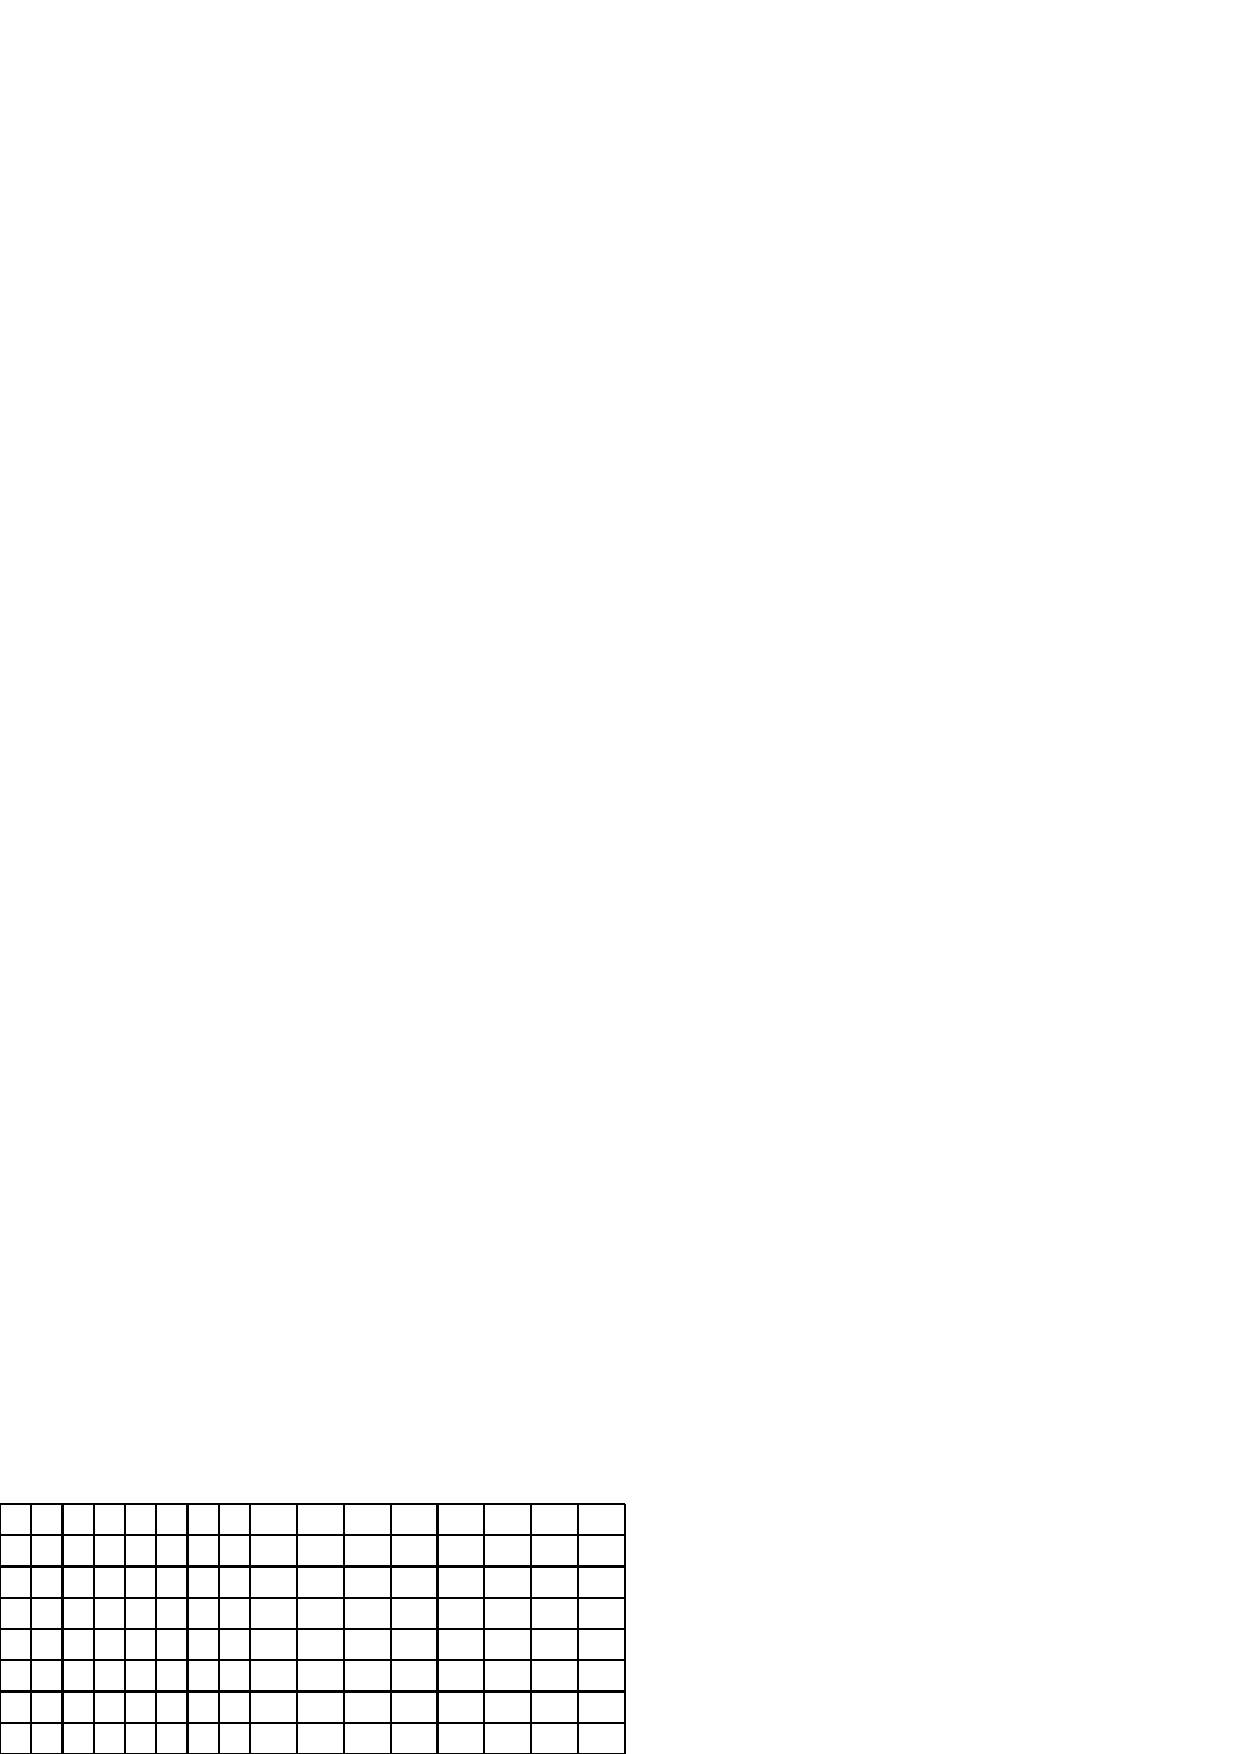
\includegraphics[width=0.45\textwidth]{mesh_r3.pdf}} \;
	\subfloat[4 mesh refinements, 512 elements]{\label{fig:mesh_4}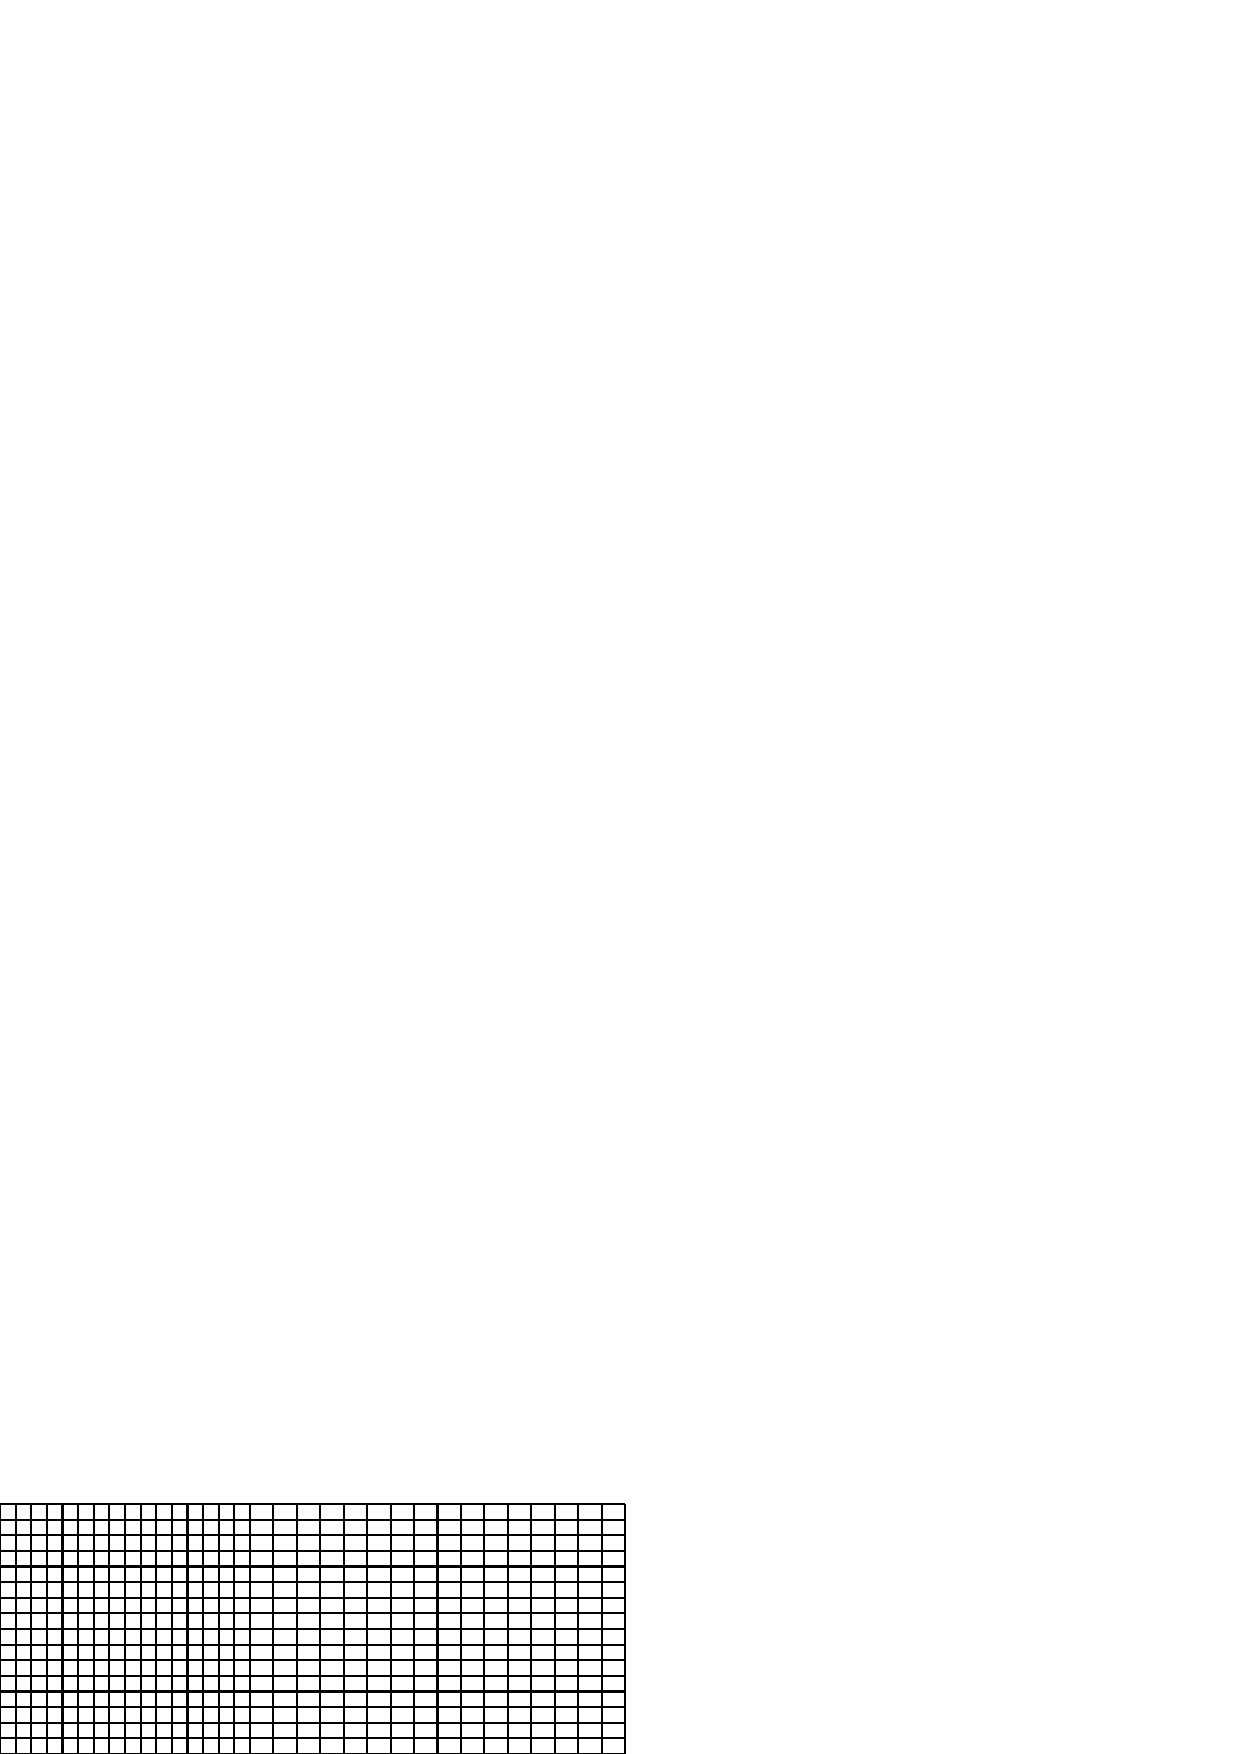
\includegraphics[width=0.45\textwidth]{mesh_r4.pdf}}
	\caption{Resulting meshes from various levels of mesh refinements}
	\label{fig:meshs}
\end{figure}

\section{Computer Implementation of the Problem}
Using the open-source C++ finite-element library \emph{deal.II}, a program was created to implement equations \ref{equ:Kij_quad}, \ref{equ:Fi_quad} and \ref{equ:F1i_quad} over the meshes given in figures \ref{fig:grid_r0} and \ref{fig:meshs}. The complete source code package is included in appendix \ref{app:source} and has been successfully compiled and run using deal.II version 7.1.0 on linux (Ubuntu 12.04) compiled with UMFPACK support.

Compiling the source code begins with placing the files ``project.cc'', ``project.ucd'', and ``Makefile'' in a directory called ''hamaluik\_project'' located in a directory called ``projects'', which is itself located in the base \emph{deal.II} installation directory. Once these files are in place and all dependencies are installed (i.e., \emph{deal.II} is configured and built with UMFPACK support), entering the command ``make'' at the command line will compile and link the program.

Once the program is appropriately compiled and linked, it is run through the command line, making use of gnu-style command line options and parameters. These options and parameters are outlined in table \ref{tab:commandlineoptions}.

\begin{table}[H]
\centering
\caption{Command line options for running the program}
\label{tab:commandlineoptions}
\begin{tabular}{ll}
\hline \hline
Flag & Description \\
\hline
	-h & show the help menu \\
	-? & show the help menu \\
	-r $<n>$ & refine the coarse mesh (given in figure \ref{fig:grid_r0}) $<n>$ times \\
	-f & if this flag is specified, the mesh geometry will be saved to a .eps file for visualization \\
	-s & if this flag is specified, the program will solve the problem (it will \textbf{not} solve anything otherwise) \\
	-q $<n>$ & manually specify the number of quadrature points to use in the calculation \\
			 & (otherwise the program will automatically calculate how many are needed for accurate integral evaluations) \\
	-o $<n>$ & specify the Lagrange polynomial order (defaults to ``1''; ``-o 2'' implies quadratic elements) \\
	-x $<x>$ & change the value of $k_x$ to $<x>$ (defaults to \unit{15}{W/m\usk K}) \\
	-y $<y>$ & change the value of $k_y$ to $<y>$ (defaults to \unit{25}{W/m\usk K}) \\
	-A $<a>$ & change the value of $A$ to $<a>$ (defaults to \unit{5000}{W/m^5}) \\
	-B $<b>$ & change the value of $B$ to $<b>$ (defaults to \unit{50}{W/m^3}) \\
	-T $<t>$ & change the value of $T$ (the Dirichlet temperature) to $<t>$ (defaults to \unit{400}{K}) \\
\hline
\end{tabular}
\end{table}

In order to run the program and evaluate the model, a file called ``project.ucd'' which defines the coarse mesh illustrated in figure \ref{fig:grid_r0} must be present in the same directory as the executable. This is a simple, common-format mesh definition file that was created by hand specifically for the geometry laid out in figure \ref{fig:domain}. A choice was made to define the geometry outside of the program in this file so that changes in the scale or relative dimensions of the domain can be modified without requiring the program to be re-compiled each time a change is made (the choice to define parameters through the command line was made for the same reasons).

The project is then invoked as such:
\vspace{-6mm}
\begin{lstlisting}[numbers=none,frame=none,language=bash]
./project [options] [solution_file_name.vtk]
\end{lstlisting}
\vspace{1mm}

Where ``[options]'' is a list of flags and parameter definitions as defined in table \ref{tab:commandlineoptions} and ``[solution\_file\_name.vtk]'' is an optional argument which lets you specify what file the solution will be written to in VTK format (this defaults to plainly ``solution.vtk'').

\subsection{Examples of Use}
To facilitate understanding of how this program is executed and a given model is solved, some simple run-time examples are included here.

\subsection{Obtaining the Help Menu}
To view the help menu for the program for information on the various parameters, their effects, and default values, we call the program using the ``-h'' flag as such:
\vspace{-6mm}
\begin{lstlisting}[numbers=none,frame=none,language=bash]
./project -h
\end{lstlisting}
\vspace{1mm}

This will result in the following being printed to the screen:
\begin{verbatim}
Usage: ./project [OPTIONS] [SOLUTION.vtk]
-- Options (defaults) --
    -?            show this help menu
    -r <level>    refine the mesh <level> times (0)
    -f            write the generated mesh to file for visualization (false)
    -s            solve the problem (false)
    -q <num|auto> use <num> quadrature points for solution (or auto-calculate based on order) (auto)
    -o <order>    set the Lagrange polynomial order to <order> (1)
    -x <Kx>       set the Kx value (15)
    -y <Ky>       set the Ky value (25)
    -A <A>        set the A value (5000)
    -B <B>        set the B value (50)
    -T <temp>     set the temperature at boundary 3 (400)
\end{verbatim}

\subsubsection{Obtaining Mesh Visualizations for Various Mesh Refinement Levels}
In order to obtain the mesh illustrations provided in figures \ref{fig:grid_r0} and \ref{fig:meshs}, the following commands were used.

To produce a file called ``mesh\_r0.eps'' which visualizes the coarsest mesh possible, the following command is used:
\vspace{-6mm}
\begin{lstlisting}[numbers=none,frame=none,language=bash]
./project -f -r 0
\end{lstlisting}
\vspace{1mm}

Similary, to produce a visualization of the highest mesh refinement examined (4 mesh refinements relating to 512 elements spread throughout the domain, outputting to file ``mesh\_r4.eps''), the following command is used:
\vspace{-6mm}
\begin{lstlisting}[numbers=none,frame=none,language=bash]
./project -f -r 4
\end{lstlisting}
\vspace{1mm}

Note that in these examples, only the mesh is assembled and output for visualization --- the program does not attempt to solve anything.

\subsubsection{Solving the Problem}
The ``default problem'' is defined as solving equations \ref{equ:Kij_quad}, \ref{equ:Fi_quad} and \ref{equ:F1i_quad} over the coarse domain illustrated in figure \ref{fig:grid_r0}, using first-order Lagrange interpolation functions, setting $A=\unit{5000}{W/m^5}$ and all other constants at their values defined in section \ref{sec:definition}. This ``default problem'' can be solved with its output being saved in ``solution.vtk'' by executing the following command:
\vspace{-6mm}
\begin{lstlisting}[numbers=none,frame=none,language=bash]
./project -s
\end{lstlisting}
\vspace{1mm}

To compute a better approximation of the solution, a greater number of elements could be used (for example, 128 elements corresponding to 3 mesh refinements):
\vspace{-6mm}
\begin{lstlisting}[numbers=none,frame=none,language=bash]
./project -r 3 -s
\end{lstlisting}
\vspace{1mm}

Using the same mesh refinement level as above, but this time investigating p-refinement, the Lagrange polynomial order can be increased so the elements are quadratic in nature:
\vspace{-6mm}
\begin{lstlisting}[numbers=none,frame=none,language=bash]
./project -r 3 -o 2 -s
\end{lstlisting}
\vspace{1mm}

Assuming this level of refinement is acceptable, we can experiment with changing the value of $A$ as part of a parametric study, outputting the solution for a given $A$ to different files for later post-processing and analysis. The following commands will generate a total of 6 different solution files, each one exploring a different value for the constant $A$ ranging from \unit{0}{W/m^5} -- \unit{5000}{W/m^5} while using a mesh with 128 linear elements.
\vspace{-6mm}
\begin{lstlisting}[numbers=none,frame=none,language=bash]
./project -r 3 -s -A 0 solution_a0k.vtk
./project -r 3 -s -A 1000 solution_a1k.vtk
./project -r 3 -s -A 2000 solution_a2k.vtk
./project -r 3 -s -A 3000 solution_a3k.vtk
./project -r 3 -s -A 4000 solution_a4k.vtk
./project -r 3 -s -A 5000 solution_a5k.vtk
\end{lstlisting}
\vspace{1mm}

A drastic alteration of the posited problem can also be solved without having to recompile or refactor the code (for example, using a finer mesh with higher-order elements, no heat generation throughout the domain, heat flux entering into the domain along boundary 1, radically different conduction coefficients, and a radically different temperature along boundary 3):
\vspace{-6mm}
\begin{lstlisting}[numbers=none,frame=none,language=bash]
./project -r 6 -o 3 -f -s -A 0 -B -1000 -x 5 -y 1 -T 0
\end{lstlisting}
\vspace{1mm}

\section{Convergence Studies}
In order to study the effect of h and p refinement on the solution, a single point in the problem domain was selected which represented a large gradient location in the solution based off of an initial higher level of refinement where the mesh was refined 4 times resulting in 512 elements and used 2nd order Lagrange interpolation polynomials (2,145 degrees of freedom). The location of this point is at \unit{(2,0.35)}{m} and can be visualized as the white cross in figure \ref{fig:refinepoint}.

\begin{figure}[H]
	\centering
	\includegraphics[width=0.75\textwidth]{refinepoint.png}
	\caption{Location of temperature probe for mesh refinement studies}
	\label{fig:refinepoint}
\end{figure}

\subsection{H-Refinement}
\label{sec:h_refine}
To study the effect of h-refinement on the solution (that is, the effect of using greater numbers of smaller elements to approximate the solution), the temperature at the given point was calculated using meshes of varying densities as illustrated in figures \ref{fig:grid_r0} and \ref{fig:meshs} using linear Lagrange interpolation elements. The temperature of the selected point was then plotted as a function of the number of degrees of freedom in the model to obtain the convergence plot illustrated in figure \ref{fig:h_refinement}.

\begin{figure}[H]
	\centering
	\includegraphics[width=\textwidth]{h_refinement.pdf}
	\caption{H-Refinement of problem}
	\label{fig:h_refinement}
\end{figure}

As can be seen in figure \ref{fig:h_refinement}, increasing the mesh density (and subsequently, the number of degrees of freedom) results in an increased temperature up to a point. It is extremely important to note the ``law of diminishing returns'' here --- once the number of degrees of freedom reaches a certain level, refining the mesh will provide no significant change in the temperature at the queried point. In this model, this point happens with approximately 3 h-refinements resulting in 128 elements or 153 degrees of freedom. We can see very plainly from this plot that nearly quadrupling the number of degrees of freedom past this point will not significantly change the approximated temperature distribution in the domain. Therefore, we can say that the model has sufficiently converged after 3 h-refinements, or with 153 degrees of freedom approximating the temperature distribution.

\subsection{P-Refinement}
To study the effect of p-refinement on the solution (that is, the effect of using higher-order Lagrange interpolation polynomials to approximate the solution), the temperature at the given point was calculated using polynomials of order 1 -- 4 for various levels of h-refinement (the same h-refinements that were performed in section \ref{sec:h_refine}). The temperature of the selected point was then plotted as a function of the number of degrees of freedom resulting in the model (higher order Lagrange interpolation polynomials result in larger numbers of degrees of freedom) to obtain the plot illustrated in figure \ref{fig:p_refinement}.

\begin{figure}[H]
	\centering
	\includegraphics[width=\textwidth]{p_refinement.pdf}
	\caption{P-Refinement of problem}
	\label{fig:p_refinement}
\end{figure}

As can be seen in figure \ref{fig:p_refinement}, increasing the polynomial order (and subsequently, the number of degrees of freedom) had no significant effect on the approximative power of the model. In fact, the only convergence of the problem was found through h-refinement, suggesting that p-refinement is not only not useful for this problem, but is also detrimental as it only serves to increase the number of degrees of freedom (and subsequently, the solution time) while doing nothing to increase the approximative power of the model.

\section{Parametric Study on the Effect of $A$}
Using 128 linear Lagrange elements resulting in 153 degrees of freedom throughout the domain, the effect of varying the constant $A$ from \unit{0}{W/m^5} -- \unit{5000}{W/m^5} was examined. Examining the temperature distribution across a constant temperature scale, the progressive change of the temperature due to progressive changes in $A$ can be visualized. The result of this analysis is presented in figure \ref{fig:paraconst}.

\begin{figure}[H]
	\centering
	\subfloat[$A=\unit{0}{W/m^5}$]{\label{fig:csa0}\includegraphics[width=0.5\textwidth]{cscale_sol_r3_o1_a0k.png}} 
	\subfloat[$A=\unit{1000}{W/m^5}$]{\label{fig:csa1}\includegraphics[width=0.5\textwidth]{cscale_sol_r3_o1_a1k.png}} \\
	\subfloat[$A=\unit{2000}{W/m^5}$]{\label{fig:csa2}\includegraphics[width=0.5\textwidth]{cscale_sol_r3_o1_a2k.png}} 
	\subfloat[$A=\unit{3000}{W/m^5}$]{\label{fig:csa3}\includegraphics[width=0.5\textwidth]{cscale_sol_r3_o1_a3k.png}} \\
	\subfloat[$A=\unit{4000}{W/m^5}$]{\label{fig:csa4}\includegraphics[width=0.5\textwidth]{cscale_sol_r3_o1_a4k.png}} 
	\subfloat[$A=\unit{5000}{W/m^5}$]{\label{fig:csa5}\includegraphics[width=0.5\textwidth]{cscale_sol_r3_o1_a5k.png}} \\
	\caption{Effect of varying $A$ on temperature distribution (with constant scale)}
	\label{fig:paraconst}
\end{figure}

As figure \ref{fig:paraconst} shows, as we increase the coefficient of the heat generation term, the problem domain experiences a a more significant temperature distribution, with the greatest temperature being concentrated in the bottom-right corner of the domain. This is to be expected as the heat generation term goes as $x^2$ (so the right side of the domain will generate significantly more heat than the left side) while there are adiabatic conditions along the bottom and right boundaries of the model. Further, this high temperature is concentrated along the bottom of the domain due to the prescribed temperature of \unit{400}{K} given at boundary 3 (along the right-top edge of the model).

For more detailed information about the temperature distribution throughout the domain, the results can be examined using different temperature scales for each value of $A$, as shown in figure \ref{fig:para}.

\begin{figure}[H]
	\centering
	\subfloat[$A=\unit{0}{W/m^5}$]{\label{fig:sa0}\includegraphics[width=0.5\textwidth]{sol_r3_o1_a0k.png}} 
	\subfloat[$A=\unit{1000}{W/m^5}$]{\label{fig:sa1}\includegraphics[width=0.5\textwidth]{sol_r3_o1_a1k.png}} \\
	\subfloat[$A=\unit{2000}{W/m^5}$]{\label{fig:sa2}\includegraphics[width=0.5\textwidth]{sol_r3_o1_a2k.png}} 
	\subfloat[$A=\unit{3000}{W/m^5}$]{\label{fig:sa3}\includegraphics[width=0.5\textwidth]{sol_r3_o1_a3k.png}} \\
	\subfloat[$A=\unit{4000}{W/m^5}$]{\label{fig:sa4}\includegraphics[width=0.5\textwidth]{sol_r3_o1_a4k.png}} 
	\subfloat[$A=\unit{5000}{W/m^5}$]{\label{fig:sa5}\includegraphics[width=0.5\textwidth]{sol_r3_o1_a5k.png}} \\
	\caption{Effect of varying $A$ on temperature distribution}
	\label{fig:para}
\end{figure}

As can be seen in figure \ref{fig:para}, when $A$ is not \unit{0}{W/m^5} the temperature distribution assumes an identical shape distribution, with only the magnitude of the temperature changing. However, as can be seen in figure \ref{fig:sa0}, when there is 0 heat generation throughout the domain, the temperature distribution is rather different, with heat visibly flowing through the domain from boundary 3 to boundary 1. In Figure \ref{fig:sa0}, it is also easy to see the effect of the variable heat flux boundary condition:
\[k_x\frac{\partial T}{\partial x} = B \left(1-y\right) \unit{}{W/m^2}\]
\noindent This shows us that there will be the greatest amount of heat flux leaving the problem domain where $y=0$ along boundary 1, which is indeed the coldest location in the domain when $A=\unit{0}{W/m^5}$. For the other cases where $A > \unit{0}{W/m^5}$, it is difficult to see from the entire temperature distribution the effect of the variable heat flux condition on boundary 1 (due to the scale of the temperature ranges). However, obtaining a plot of temperature as a function of the y-coordinate along boundary 1 (where $x=0$) sheds some insight as is seen in figure \ref{fig:y_temp} (plotted for the case where $A=\unit{5000}{W/m^5}$).

\begin{figure}[H]
	\centering
	\includegraphics[width=\textwidth]{y_temp.pdf}
	\caption{Temperature profile along $y$ axis at $x=\unit{0}{m}$ when $A=\unit{5000}{W/m^5}$}
	\label{fig:y_temp}
\end{figure}

As is seen in figure \ref{fig:y_temp}, the temperature does indeed change along boundary 1. However, the temperature profile here is somewhat ``opposite'' to what is expected --- at $y=0$, we expect the lowest temperature as this is where the greatest heat flux occurs. We must look beyond this, however, and realize that the prescribed temperature of \unit{400}{K} along boundary 3 (which is at the top of the model) will ``override'' this heat flux and cause lower temperatures at the top of the model, rather than the bottom.

The effect of varying $A$ can also be considered by plotting the temperature distribution in a single dimension (in this case, the $x$ dimension) of the domain. To do this, a line going through the center of the problem domain at $y=\unit{0.5}{m}$ with $x\in\unit{(0, 2.5)}{m}$ was chosen and is illustrated in figure \ref{fig:studyline}.

\begin{figure}[H]
	\centering
	\includegraphics[width=0.75\textwidth]{studyline.png}
	\caption{Location of line along which temperature is evaluated}
	\label{fig:studyline}
\end{figure}

The temperature profile along this line was then recorded for $A$ varying between \unit{0}{W/m^5} -- \unit{5000}{W/m^5}, and is illustrated in figure \ref{fig:a_study}.

\begin{figure}[H]
	\centering
	\includegraphics[width=\textwidth]{a_study.pdf}
	\caption{Temperature profile along $x$ axis at $y=\unit{0.5}{m}$}
	\label{fig:a_study}
\end{figure}

From figure \ref{fig:a_study}, it is clear to see the effect of increasing $A$ --- as $A$ is increased, the temperature profile across the entire domain increases while the gradient effect of the $x^2$ term becomes more and more apparent. That is, the temperature gradient at higher $A$ is significantly greater than the temperature gradient at lower $A$. It is expected this is the case since at greater values of $A$, the heat-generation term in the problem has a significantly greater effect in comparison to the various boundary conditions in the model (the heat flux along the left edge and the prescribed temperature along the top) which are completely independent of $A$ and will be ``over-ridden'' by the large amount of heat generated in the domain.

\pagebreak
\appendix
\addappheadtotoc
\makeatletter
\def\@seccntformat#1{Appendix\ \csname the#1\endcsname:\ }
\makeatother
\renewcommand{\thepage}{\thesection-\arabic{page}}
\setcounter{page}{1}

\section{Source Code Listings}
\label{app:source}
\subsection{Project Source File}
\lstinputlisting[title=project.cc]{../project.cc}
\subsection{Geometry Definition File}
\lstinputlisting[title=project.ucd]{../project.ucd}
\subsection{Makefile}
\lstinputlisting[title=Makefile,language=make]{../Makefile}

\pagebreak
\setcounter{page}{1}
\section{Declaration Form}
\begin{center}
{%
\setlength{\fboxsep}{0pt}%
\setlength{\fboxrule}{1pt}%
\fbox{\includegraphics[width=0.99\textwidth]{declaration.pdf}}%
}%
\end{center}

\end{document}
